\chapter{Enviroment and basics}
\label{cha:enviromentandbasics}

\section{Programming tools}
As the target of this thesis is a mere proof of concept, the programming language of choice is matlab \cite{tool:matlab}. This is a reasobable decision because in the matlab language a huge part of the needed functionality concerning simple mathematical functions is already implemented and easy to use. \\
Pros:
\begin{itemize}
\item easy to use mathematical function
\item fast and easy way to enter data
\item good and simple ways of debugging and locating errors 
\end{itemize}
Cons:
\begin{itemize}
\item slow computation speed
\item needs translation in other language ( e.g. c++ ) for further use
\end{itemize}

As versioning tool git \cite{tool:git} is used together with www.github.com as an open source storage plattform for the resulting code.

\section{Basics}
For better understanding of the following chapters the central mathematical formulas are repeated here.

\subsection{basic vector math} %representation with points
If the objects are represented as a list of corner points, vector math comes in handy when describing the borders of the object.
Lets say we have a simple object A defined by the following list:
\begin{align*}
A = 	&( 0 , 0 ;2 , 0 ;2, 2; 0, 2)	
\end{align*}

Each pair x,y defines one corner of A and the points are ordered to travel along the border of A counterclockwise.
The lines connecting these points will be called the borders of A. They are calculated by substracting the points from each other such that the vectors point along the border clockwise. This leads to:
\begin{align*}
A_{vec} = 	&( 2 , 0 ; 0 ,2 ;-2, 0; 0, -2)	
\end{align*}

\begin{figure}[H]
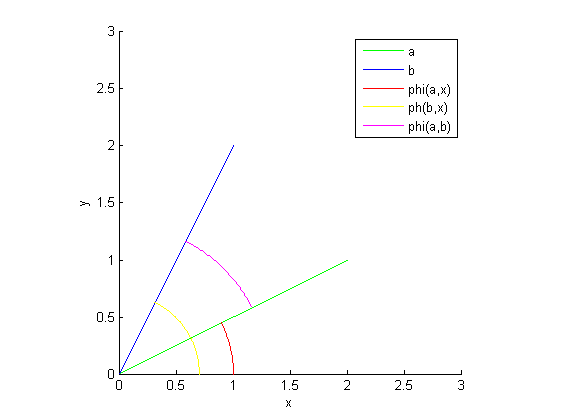
\includegraphics{VectorDegree}
\caption{Figure showing the calculation of the angle difference beetween vectors $a$ and $b$ via reference to x-axis}
 \end{figure}

Next will be the calculation of the angle beetween two lines $a$ and $b$. This is done by taking a reference vector , for example the x-axis r=$(1,0)$, calculating the angle to that and building the difference in angle. This way we can determine an angle beetween the vectors $a$ and$b$ where the sign of the angle tells us which vector lies "below" the other.\\
The formula for this is:
\begin{align*}
  \phi_{a,b} &= \phi_{a,r} - \phi_{b,r}\\
	&= tan^{-1} ( \frac{ a(2) }{  a(1) } ) - tan^{-1} ( \frac{b(2)}{b(1)}); 
\end{align*}
We need to use another vector as a reference to determine if the vectors angle difference is positiv or negativ. This information is needed to build the convex hull.

\subsection{convex hull} %collision representation with points
Next is the calculation of the convex hull of an object for another object. Lets take object A from before and another object B defined by:
\begin{align*}
B = 	&( 0 , 0 ;1 , 0 ;1, 2; 0, 2)	
\end{align*}
Furthermore we define the center of these objects to be $M_A = (1,1)$ and $M_B = (0.5 , 1)$
The convex hull for A to B is calculated after the formula
\begin{align*}
	hull &= formula
\end{align*}
Basically this means we add the points of A shifted with $-M_A$ and mirrored at $M_A$ to each point of B shifted with $-M_B$ and then reshifted with $M_B$ to get a list $C_{temp}$ of $4\cdot 4 = 16$  points.
\begin{align*}
C_{temp} =	\begin{matrix}
		(&-1, &-1; &1, &-1; &1, &1; &-1, &1;\\
		&0, &-1; &2, &-1; &2, &1; &0, &1;\\
		&0, &1; &2, &1; &2, &3; &0, &3;\\
		&-1, &1; &1, &1; &1, &3; &-1, &3)
		\end{matrix}
\end{align*}
Each line represents one point of B with the points of A added. By choosing the outer points from $C_{temp}$ and put them in $C$, such that no point from $C_{temp}$ is still outside $C$  we will get an object C which defines the space around B which the object A can not enter or they will collide.
\begin{align*}
C = (-1,-1; 2, -1; 2 ,3; -1, 3)
\end{align*}
